\begin{figure}[H]
\centering
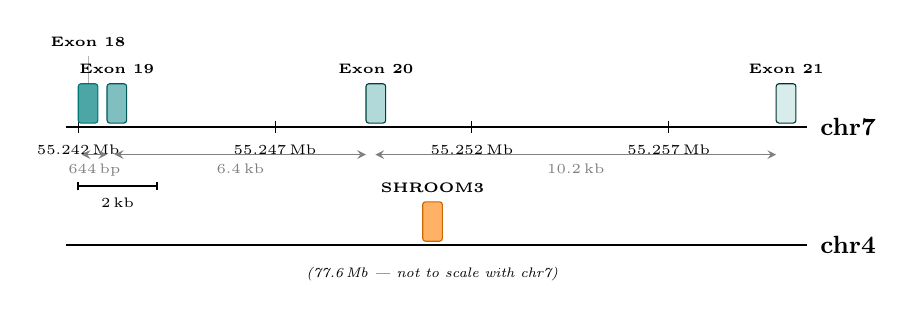
\begin{tikzpicture}[x=0.5cm, y=1cm, font=\footnotesize]

  % ---- chr7 axis ----
  % Coordinates in kb, offset from 55,241,646 (= 0 kb)
  % Amp1 (ex18): 0.000–0.088 kb   Amp2 (ex19): 0.732–0.928 kb
  % Amp3 (ex20): 7.310–7.548 kb   Amp4 (ex21): 17.728–17.943 kb

  % chromosome backbone
  \draw[thick] (-0.3, 0) -- (18.5, 0);
  \node[right, font=\small\bfseries] at (18.6, 0) {chr7};

  % kb tick marks every 5 kb with Mb labels
  \foreach \kb/\lbl in {0/55.242, 5/55.247, 10/55.252, 15/55.257} {
    \draw (\kb, 0.08) -- (\kb, -0.08);
    \node[below, font=\tiny] at (\kb, -0.1) {\lbl\,Mb};
  }

  % amplicons — drawn with min display width 0.5 kb; actual widths are 88–238 bp
  % colours: teal shades for EGFR amplicons
  \filldraw[fill=teal!70, draw=teal!90!black, rounded corners=1pt]
    (0.000, 0.05) rectangle (0.50, 0.55);
  \filldraw[fill=teal!50, draw=teal!70!black, rounded corners=1pt]
    (0.732, 0.05) rectangle (1.23, 0.55);
  \filldraw[fill=teal!30, draw=teal!50!black, rounded corners=1pt]
    (7.310, 0.05) rectangle (7.81, 0.55);
  \filldraw[fill=teal!15, draw=teal!40!black, rounded corners=1pt]
    (17.728, 0.05) rectangle (18.23, 0.55);

  % amplicon labels above — Exon 18 raised to avoid overlap with Exon 19
  \node[above, font=\tiny\bfseries] at (0.25,  0.90) {Exon 18};
  \draw[gray!60, thin] (0.25, 0.56) -- (0.25, 0.90);
  \node[above, font=\tiny\bfseries] at (0.98,  0.55) {Exon 19};
  \node[above, font=\tiny\bfseries] at (7.56,  0.55) {Exon 20};
  \node[above, font=\tiny\bfseries] at (17.98, 0.55) {Exon 21};

  % ---- gap annotations below axis ----
  % Gap A1→A2: 0.088 → 0.732 = 644 bp
  \draw[<->, >=stealth, gray] (0.088, -0.35) -- (0.732, -0.35);
  \node[below, gray] at (0.41, -0.35) {\tiny 644\,bp};

  % Gap A2→A3: 0.928 → 7.310 = 6,382 bp
  \draw[<->, >=stealth, gray] (0.928, -0.35) -- (7.310, -0.35);
  \node[below, gray] at (4.12, -0.35) {\tiny 6.4\,kb};

  % Gap A3→A4: 7.548 → 17.728 = 10,180 bp
  \draw[<->, >=stealth, gray] (7.548, -0.35) -- (17.728, -0.35);
  \node[below, gray] at (12.64, -0.35) {\tiny 10.2\,kb};

  % ---- scale bar ----
  \draw[thick] (0, -0.75) -- (2, -0.75);
  \draw[thick] (0, -0.70) -- (0, -0.80);
  \draw[thick] (2, -0.70) -- (2, -0.80);
  \node[below] at (1, -0.78) {\tiny 2\,kb};

  % ---- chr4 (separate chromosome, schematic only) ----
  \draw[thick] (-0.3, -1.5) -- (18.5, -1.5);
  \node[right, font=\small\bfseries] at (18.6, -1.5) {chr4};
  \node[below, font=\tiny] at (9.0, -1.65) {\textit{(77.6\,Mb — not to scale with chr7)}};

  % SHROOM3 — positioned at centre for schematic representation
  \filldraw[fill=orange!60, draw=orange!80!black, rounded corners=1pt]
    (8.75, -1.45) rectangle (9.25, -0.95);
  \node[above, font=\tiny\bfseries] at (9.0, -0.95) {SHROOM3};
  \node[below, font=\tiny] at (9.0, -1.65) {};

\end{tikzpicture}
\caption{Relative genomic positions of the five covered intervals on chr7 and chr4 (hg19).
  The chr7 axis is drawn to scale: the four EGFR amplicons span $\sim$18\,kb in total,
  with a 644\,bp gap between exons~18 and~19, a 6.4\,kb gap to exon~20, and a 10.2\,kb gap
  to exon~21. Amplicon widths are exaggerated for visibility (actual widths 88--238\,bp).
  The chr4 SHROOM3 interval (77.6\,Mb) is shown schematically and is not to scale
  relative to chr7.}
\label{fig:amplicon-positions}
\end{figure}
